% The generic preamble
\documentclass[10pt,letterpaper,fleqn,titlepage]{article}

% Define packages to use
\usepackage{natbib}
\usepackage[dvips]{graphicx,color}
\usepackage{amsmath,amssymb}
\usepackage{bm}
\usepackage{caption}
\usepackage{xr}
\usepackage{ifthen}
\usepackage[dvipdfm,colorlinks,linkcolor=blue,citecolor=blue,urlcolor=blue]{hyperref}
\usepackage{fancybox}
\usepackage{textcomp}
\usepackage{alltt}
%\usepackage{floatflt}
%\usepackage{svn}


% Redefine default page
\setlength{\textheight}{9in}  % 1" above and below
\setlength{\textwidth}{6.75in}   % 0.5" left and right
\setlength{\oddsidemargin}{-0.25in}

% Redefine default paragraph
\setlength{\parindent}{0pt}
\setlength{\parskip}{1ex plus 0.5ex minus 0.2ex}

% Define caption width and default fonts
\setlength{\captionmargin}{0.5in}
\renewcommand{\captionfont}{\sffamily}
\renewcommand{\captionlabelfont}{\bfseries\sffamily}

% Define commands for super- and subscript in text mode
\newcommand{\superscript}[1]{\ensuremath{^\textrm{#1}}}
\newcommand{\subscript}[1]{\ensuremath{_\textrm{#1}}}

% Derived commands
\newcommand{\invcm}{\textrm{cm\superscript{-1}}}
\newcommand{\micron}{\ensuremath{\mu\textrm{m}}}

\newcommand{\df}{\ensuremath{\delta f}}
\newcommand{\Df}{\ensuremath{\Delta f}}
\newcommand{\dx}{\ensuremath{\delta x}}
\newcommand{\Dx}{\ensuremath{X_{max}}}
\newcommand{\Xeff}{\ensuremath{X_{eff}}}

\newcommand{\water}{\textrm{H\subscript{2}O}}
\newcommand{\carbondioxide}{\textrm{CO\subscript{2}}}
\newcommand{\ozone}{\textrm{O\subscript{3}}}

\newcommand{\taup}[1]{\ensuremath{\tau_{#1}}}
\newcommand{\efftaup}[1]{\ensuremath{\tau_{#1}^{*}}}

\newcommand{\textbfm}[1]{\boldmath\ensuremath{#1}\unboldmath}

\newcommand{\rb}[1]{\raisebox{1.5ex}[0pt]{#1}}

\newcommand{\f}[1]{\texttt{#1}}

% Define how equations are numbered
\numberwithin{equation}{section}
\numberwithin{figure}{section}
\numberwithin{table}{section}

% Define a command for title page author email footnote
\newcommand{\email}[1]
{%
  \renewcommand{\thefootnote}{\alph{footnote}}%
  \footnote{#1}
  \renewcommand{\thefootnote}{\arabic{footnote}}
}

% Define a command to print the Office Note subheading
\newcommand{\notesubheading}[1]
{%
  \ifthenelse{\equal{#1}{}}{}
  { {\Large\bfseries Office Note #1\par}%
    {\scriptsize \sc This is an unreviewed manuscript, primarily intended for informal}\\ 
    {\scriptsize \sc exchange of information among JCSDA researchers\par}%
  }
}

% Redefine the maketitle macro
\makeatletter
\def\docseries#1{\def\@docseries{#1}}
\def\docnumber#1{\def\@docnumber{#1}}
\renewcommand{\maketitle}
{%
  \thispagestyle{empty}
  \vspace*{1in}
  \begin{center}%
     \sffamily
     {\huge\bfseries Joint Center for Satellite Data Assimilation\par}%
     \notesubheading{\@docnumber}
  \end{center}
  \begin{flushleft}%
     \sffamily
     \vspace*{0.5in}
     {\Large\bfseries\ifthenelse{\equal{\@docseries}{}}{}{\@docseries: }\@title\par}%
     \medskip
     {\large\@author\par}%
     \medskip
     {\large\@date\par}%
     \bigskip\hrule\vspace*{2pc}%
  \end{flushleft}%
  \newpage
  \setcounter{footnote}{0}
}
\makeatother
\docseries{}
\docnumber{}


% Define a command for a DRAFT watermark
\usepackage{eso-pic}
\newcommand{\draftwatermark}
{
  \AddToShipoutPicture{%
    \definecolor{lightgray}{gray}{.85}
    \setlength{\unitlength}{1in}
    \put(2.5,3.5){%
      \rotatebox{45}{%
        \resizebox{4in}{1in}{%
          \textsf{\textcolor{lightgray}{DRAFT}}
        }
      }
    }
  }
}




% Define included documents
\includeonly{Ocean_Height_Variance_LUT,Complex_Number_TLAD.appendix}


% Definitions for tables
\newcommand{\rb}[1]{\raisebox{1.5ex}[0pt]{#1}}
\newcommand{\po}{\ensuremath{p_{0}}}
\newcommand{\bpo}{\boldmath\po\unboldmath}
\newcommand{\Dp}{\ensuremath{\Delta p}}
\newcommand{\bDp}{\boldmath\Dp\unboldmath}
\newcommand{\reff}{\ensuremath{R_{eff}}}
\newcommand{\breff}{\boldmath\reff\unboldmath}
\newcommand{\bhpa}{\textbf{(hPa)}}
\newcommand{\bmicron}{\boldmath\micron\unboldmath}

% Title info
\title{Implementation of a Low Frequency Microwave Sea Surface Emissivity Model}
\author{Paul van Delst\email{paul.vandelst@noaa.gov}\\JCSDA/EMC/SAIC}
\date{April, 2008}
\docnumber{(unassigned)}
\docseries{CRTM}


%-------------------------------------------------------------------------------
%                            Ze document begins...
%-------------------------------------------------------------------------------
\begin{document}
\maketitle

\draftwatermark

\begin{abstract}
The implementation of M.Kazumori's low frequency microwave sea surface emissivity model, for use with the AMSR-E instrument, involved refactoring some existing code.

\textbf{Keywords}: CRTM, microwave sea surface emissivity
\end{abstract}


\section{Introduction}
%=====================
blah blah blah

% Include all the other various sections
%=======================================
\section{Ocean Height Variance Lookup Table}
%===========================================

\begin{figure}[htp]
  \centering
  \includegraphics[scale=0.8]{graphics/LUT/sdd_sfc.eps}
  \caption{Ocean height variance as a function of frequency (GHz) and wind speed (m.s\superscript{-1}) used in the emissivity model LUT.}
  \label{fig:sdd_sfc}
\end{figure}

\begin{figure}[htp]
  \centering
  \includegraphics[scale=0.8]{graphics/LUT/sdd_frequency_spectra.eps}
  \caption{Ocean height variance frequency spectra for each wind speed (m.s\superscript{-1}) used in the emissivity model.}
  \label{fig:sdd_frequency_spectra}
\end{figure}

\begin{figure}[htp]
  \centering
  \includegraphics[scale=0.8]{graphics/LUT/sdd_wind_speed_spectra.eps}
  \caption{Ocean height variance wind speed spectra for each frequency (GHz) used in the emissivity model.}
  \label{fig:sdd_wind_speed_spectra}
\end{figure}






\section{Conclusions}
%====================
blah blah blah
\cite{Guillou_etal_1998}

% The references section
%=======================
\bibliographystyle{plain}
\bibliography{bibliography}	


% The appendices section
%=======================
\begin{appendix}
  \section{Testing the tangent-linear and adjoint of complex numbered expressions}
%===============================================================================

Given a complex number, $z$, such that,
\begin{equation}
  z = a + ib
  \label{eqn:z_defn}
\end{equation}
where $i = \sqrt{-1}$, let a real number, $r$, be the square of the absolute value of $z$,
\begin{equation}
  r = |z|^2
  \label{eqn:r_z}
\end{equation}
This can be rewritten as,
\begin{equation}
  r = z.\overline{z}
  \label{eqn:r_zconjz}
\end{equation}
where $\overline{z}$ is the complex conjugate,
\begin{equation}
  \overline{z} = a - ib
  \label{eqn:conjz_defn}
\end{equation}
The tangent-linear form of equation \ref{eqn:r_zconjz} is written as,
\begin{equation}
  \delta r = 2z.\delta\overline{z}
  \label{eqn:r_zconjz_tl}
\end{equation}
The adjoint form of equation \ref{eqn:r_zconjz_tl} is,
\begin{equation}
  \delta^{*}\overline{z} = 2z.\delta^{*}r
  \label{eqn:r_zconjz_ad}
\end{equation}
We define a simple test where, when the tangent-linear output of equation \ref{eqn:r_zconjz_tl} is used as the adjoint input of equation \ref{eqn:r_zconjz_ad}, then
\begin{equation}
  \delta r^{T}\delta r = \delta z^T \delta^{*}\overline{z} 
  \label{eqn:r_z_tlad_test}
\end{equation}
Substituting the results of equations \ref{eqn:r_zconjz_tl} and \ref{eqn:r_zconjz_ad} into equation \ref{eqn:r_z_tlad_test} we get,
\begin{eqnarray}
  \left(2z.\delta\overline{z}\right)^{2} & = & \delta\overline{z}.2z.\delta r\nonumber \\
                                         & = & \delta\overline{z}.2z.2z.\delta\overline{z}\nonumber \\
                                         & = & \left(2z.\delta\overline{z}\right)^{2}
  \label{eqn:r_z_tlad_test_subst}
\end{eqnarray}
where the transpose of a complex number is also its conjugate. The latter follows if one represents a complex number as an antisymmetric matrix,
\begin{equation}
  z \equiv \left[
             \begin{array}{c c}
               a & -b \\
               b & a
             \end{array}
           \right]
\end{equation}
where it is clear that $z^T = \overline{z}$.

\end{appendix}


\end{document}

